\begin{itemize}
	\item Das Interface wird aus �ffentlichen Funktionen bestehen, die im Release-Modus nichts tun und im Debug-Modus, so gew�nscht, die nicht-�ffentlichen Debug-Methoden aufrufen.
	\item Die nicht�ffentlichen Debug-Funktionen erzeugen eine graphische Visalisierung und f�gen diese dem
	Thread-lokalen Hauptfenster hinzu.
	\item Die Bibliothek selbst wird �ber die Funktionen des �ffentliche Userinterfaces angesteuert die lediglich pr�fen ob der Debugmodus aktiv ist und gegebenenfalls die eigentlichen Funktionen im nicht�ffentlichen, technischen Interface aufrufen.
\end{itemize}


\begin{figure}[H]
\centering
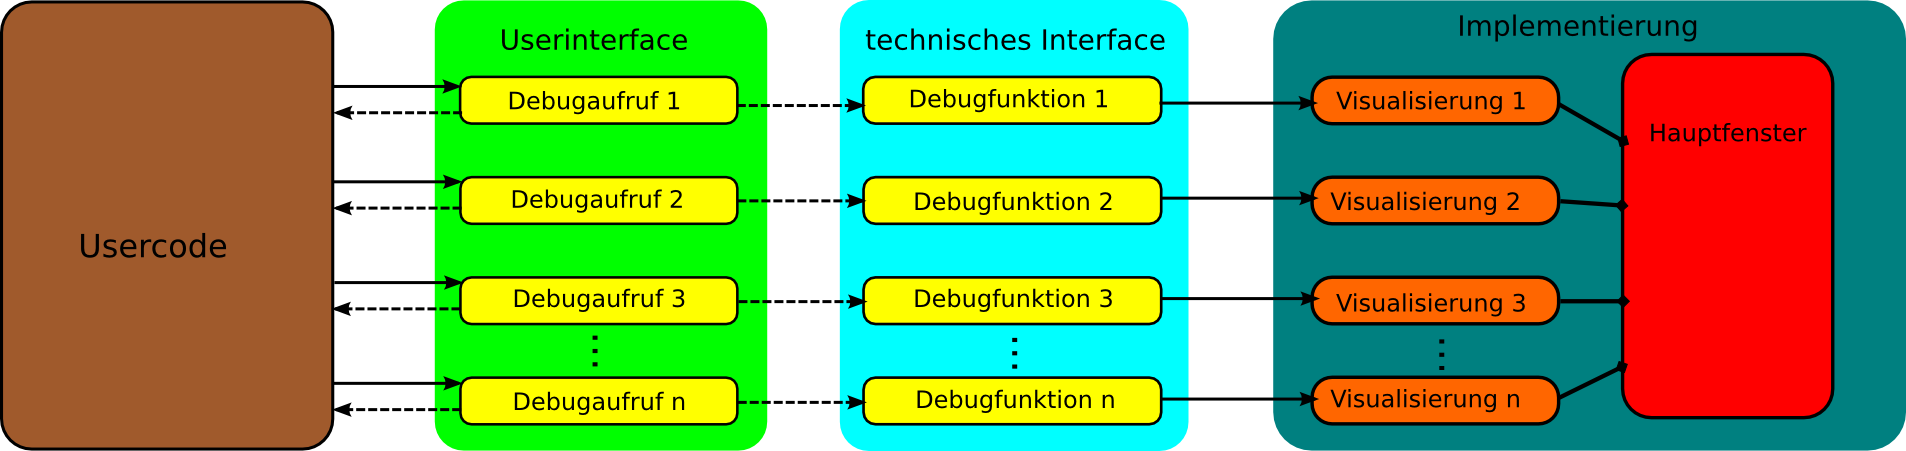
\includegraphics[width=\linewidth]{../architektur_skizze}
\caption[Das Modul besteht aus drei Layern bei denen jeweils die �u�eren die Inneren aufrufen]{Das Modul besteht aus drei Layern bei denen jeweils die �u�eren die Inneren aufrufen}
\label{fig:architektur_skizze}
\end{figure}
